\textbf{Danke an ...}
\\

\begin{tabular}{l l l} 

Adrian Ackermann & Tim Kluge & Josephine Rehak\\
Justus Adam & Fabian Koller & Axel Reinicke\\
Anna Baumgärtel & Kilian Költzsch & Franziska Ressel\\
Bettina Blasberg & Nadja Konrad & Anja Reusch\\
Meinhardt Branig & Max Korn & Christian Riedel\\
Anna Brauer & Ben Kosmann & Christian Rose\\
Markus Damm & Nikolai Kostka & Marcel Rösler\\ 
Felix Döring & Alexandra Krien & Marc Satkowski\\ 
Georg Eckert & Sandra Kukulka & Florian Schmidt\\
Björn Einert & Richard Kwasnicki & Michael Schneider\\
Martin Eisoldt & Kristian Kyas & Lara von Schumann\\
Lars Engeln & Dirk Legler & Franz-Wilhelm Schumann\\
Daniel Fischer & Matthias Lehne & Franziska Schwenke\\ 
Tamara Flemisch & Adrian Lieber & Rico Skultety\\
Sven Goly & Katja Linnemann & Patrick Stiller\\
Julius Gonsior & Ian Alexander List & Julian Lars Striegl\\
Sara Groß & Willi Mentzel & Sinthujan Thanabalasingam\\
Anita Grützner & Sebastian Mielke & Manuel Thieme\\
Sebastian Hahn & Richard Mörbitz & Duc Anh Trinh\\
Thomas Hauptvogel & Emma Müller & Sebastian Vogt\\
Frank Hedecke & Vincent Nadoll & Sandra Waske\\
Philipp Heisig & Anne-Marie Oelschläger & Stefan Weckend\\
Marius Hogräfer & David Ordnung & Jens Wettlaufer\\
Ulrich Huber & Dominik Pataky & Andreas Wilke\\
Christoph Jurkowski & Sascha Peukert & Lucas Woltmann\\
Christian Kabelitz & Philipp Plotz & Laura Zepner\\
Sebastian Kiehne & Lisa Ragosina & \\
Peter Klausing & Melanie Ramsch & \\

\end{tabular}

\addchap{Vorwort}

Hallo Uniwelt!

heißt es nun für dich als frisch Immatrikulierter, Ersti, an der TU Dresden. 
Endlich kannst du nach Jahren der Knechtschaft selbst über dich und dein Leben bestimmen. 
Wie du mit dieser Freiheit und der daraus folgenden Verantwortung zurecht kommst, lernst du schnell. 
Damit dir der Übergang leichter fällt, veranstaltet dein Fachschaftsrat die Erstsemestereinführung (ESE). 
Eine Woche lang gibt es neben Spiel und Spaß sehr viel Informatives zum Studium sowie zum Unileben allgemein. 
Dieses Heft ist ein nützlicher Ratgeber und nicht vergessen: 
\textbf{NO PANIC!} (Aus historischen Gründen hier nicht das grammatikalisch korrekte \glqq don't panic\grqq. Hinweise auf diesen grammatikalischen Fauxpas werden mit Matekästenschulden geahndet.)

Du wirst auch entdecken, dass Uni mehr ist als nur studieren. 
Neben allerlei Erstsemesterparties gibt es noch mehr zu erleben. 
Gerade prägend für die Dresdner Hochschulkultur sind die 17 Studentenclubs, wie z.B. das CountDown in der Johannstadt. 
In der Neustadt laden ebenso viele Kneipen und Clubs zu langen Nächten ein. 
Einmal im Jahr entlädt sich dieses alternative Flair während der BRN (Bunte Republik Neustadt). 
Und wem das alles viel zu hektisch ist: der fläze sich gemütlich in ein Sofa vom ASCII, dem Studentencafé der Fakultät. 
Dort kann man gut bei Kaffee und Club Mate (empfehlenswert auch die lokale Kolle-Mate!) entspannen oder versuchen doch etwas für die Uni zu tun.

Engagement wird an der TU Dresden groß geschrieben. 
Es gibt viele Hochschulgruppen die um eure Mitarbeit buhlen. 
Darunter einige politische, wie auch technische, journalistische, künstlerische und und und. Mehr dazu findest du auf der Seite des Studentenrates (StuRa).

Dieses Heft enthält übrigens auch eine Vielzahl von Links zu relevanten Unterseiten auf den Seiten des Fachschaftsrates (FSR), der Uni und anderen. 
Diese sind mit Zahlen wie dieser hier \link{http://html5zombo.com} versehen und ganz am Ende des Heftes gelistet. Ebenfalls kannst du auch direkt unter \url{ese.ifsr.de/2014/<Zahl>} auf die verlinkte Seite weitergeleitet werden.

\textbf{Zu guter Letzt: Wir (deine ESE-Tutoren) wünschen dir viel Erfolg und auch ordentlich Spaß beim Studium!}

\begin{figure}
\centering 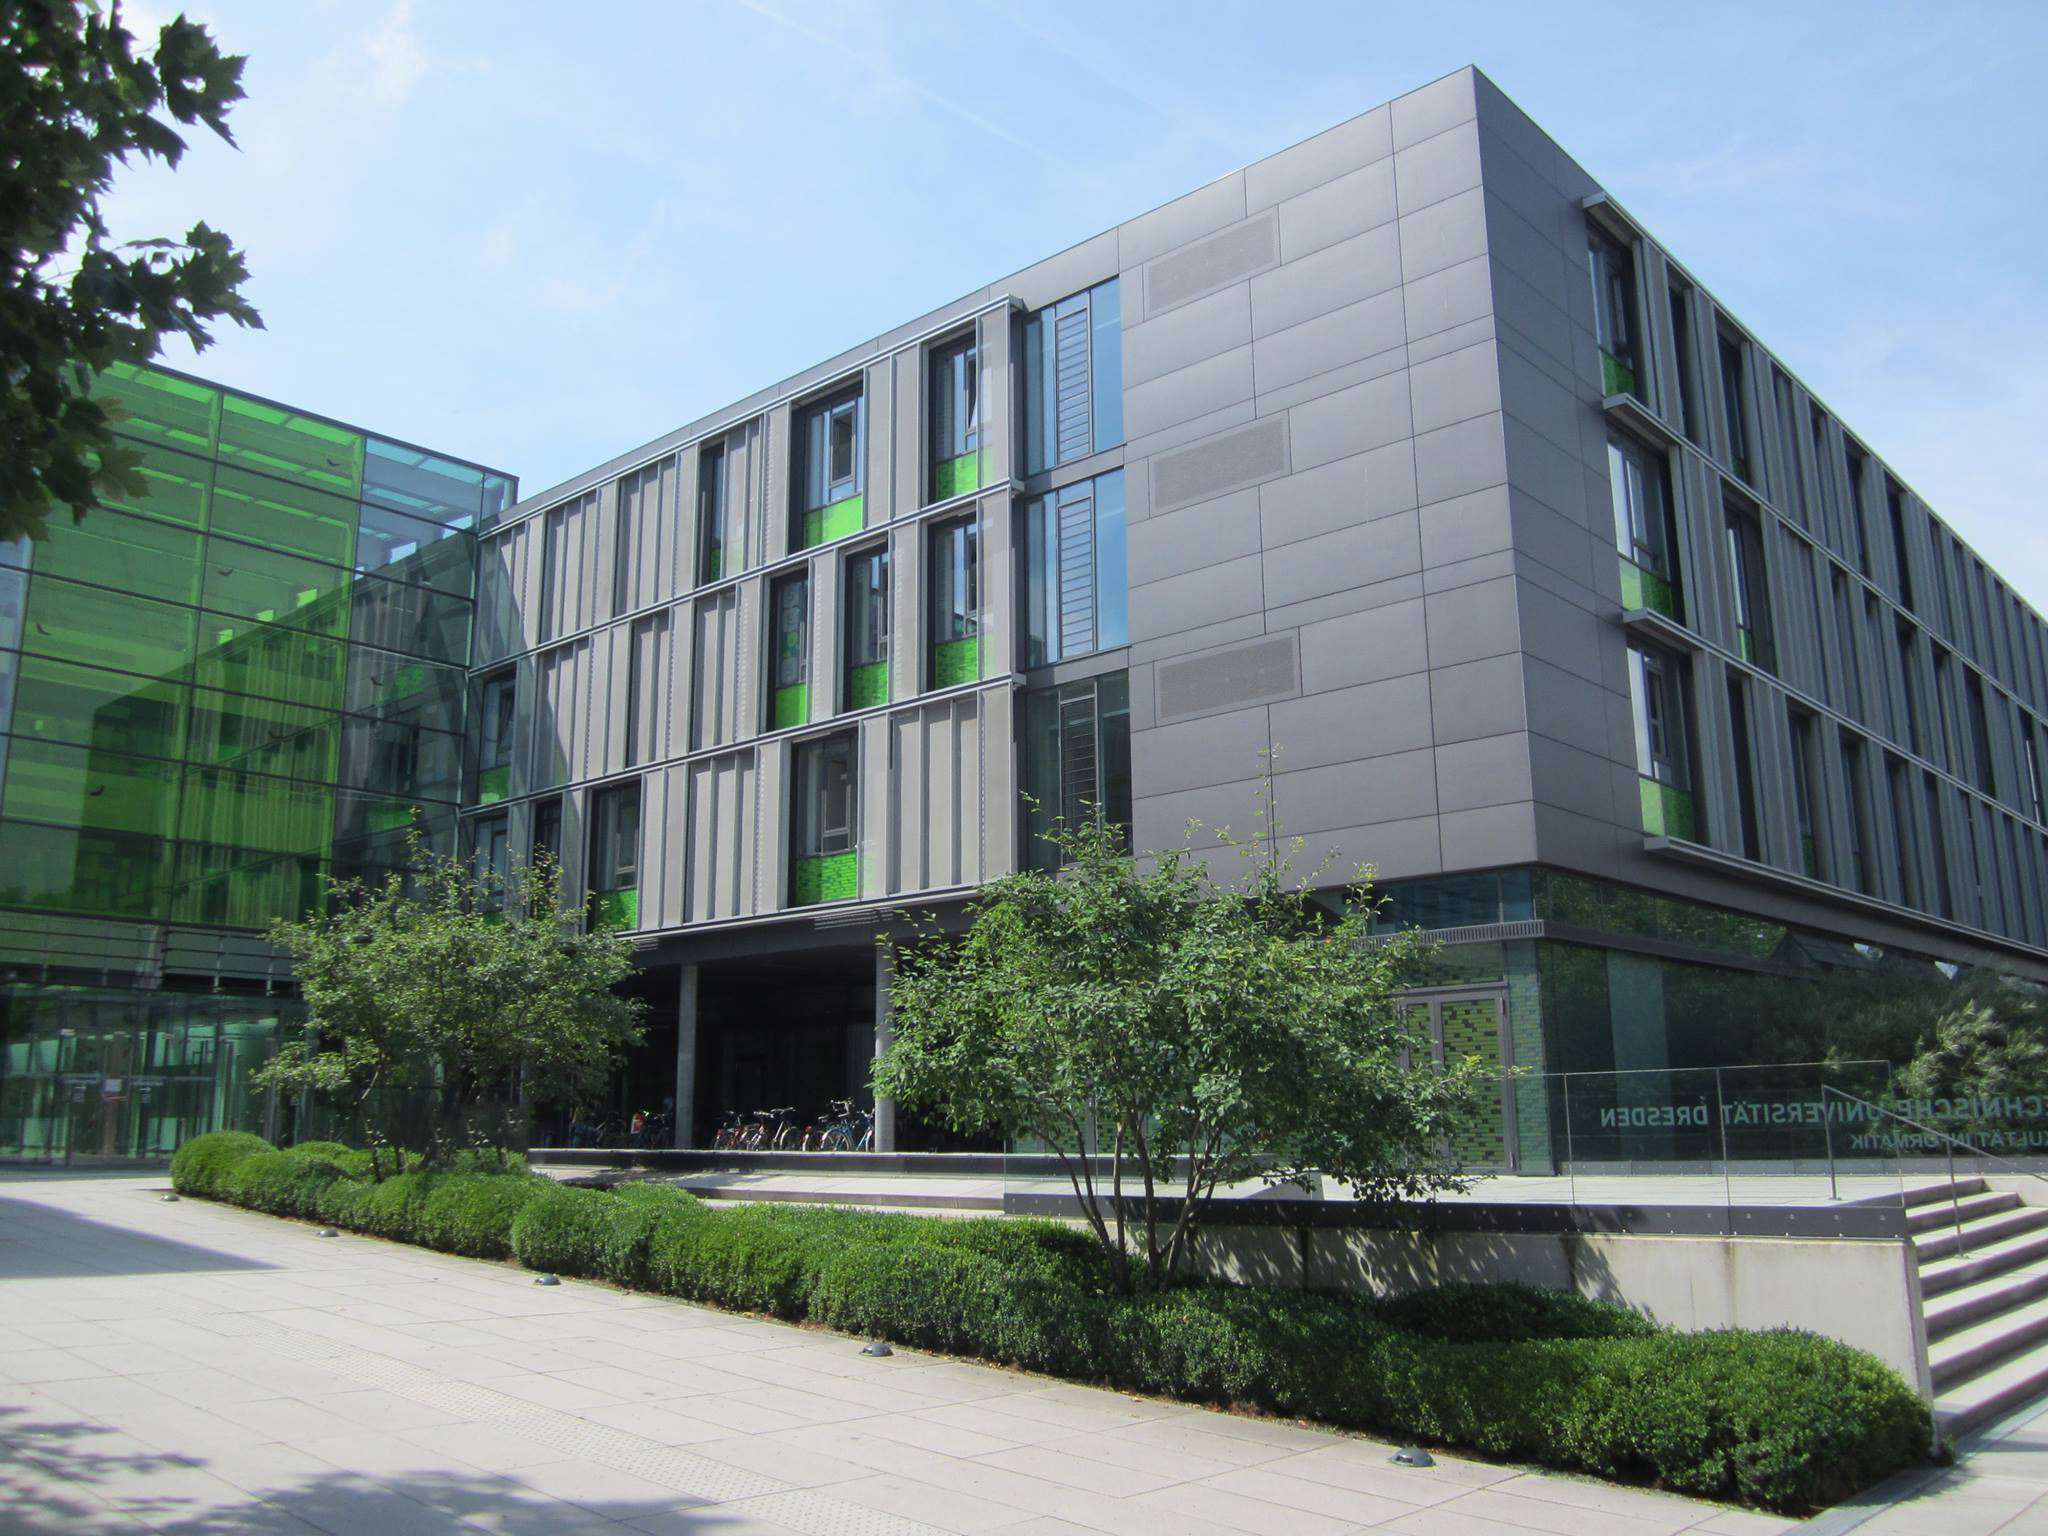
\includegraphics[width=\linewidth]{img/fakultaet.jpg}
\caption*{{\small Andreas-Pfitzmann-Bau (Fakultät Informatik) - Foto: Philipp Heisig}}
\end{figure}
%Bildlink: http://commons.wikimedia.org/wiki/File:TU-Dresden-Informatik.jpg
